\chapter{Results}
\label{chp:res}
In order to verify the proposed method, we test it with data obtained from two different testbeds. First, we apply our method to the data collected from the test bed which is described in chapter \ref{chp:testbed}. Next, we make use of the data released by the WSU smart home project\footnote{http://ailab.wsu.edu/casas/datasets/} \cite{cook2009assessing}. We use C++ implementation of the VF2 algorithm released by the authors available at \cite{vfLib} for finding the mappings between the grid graph and the MST of correlation Matrix $(R)$.
\section{Error Metrics }
To evaluate the results we define an error metrics as follows:\\
\begin{equation}
error=\frac{\text{Number of misplaced sensors}}{\text{Number of sensors}}
\end{equation}
\section{Data Length}
\label{sec:dataLength}
An important aspect to know in a data-driven method is, how much of data is required in order to get accurate results? To answer this question, the entire dataset of length $T$ is divided into blocks of time interval $t$ as shown in the figure \ref{fig:time}. We iteratively increment $t$ until a value beyond which error observed for all the blocks of data of length $t$ is zero. 
This is done because there can be parts of the data which might give pseudo high correlation value between two nonneighboring nodes or vice versa due to various reasons like noise in the sensor data, large period of inactivity etc. As the data length increases, the effect of the data influencing the false correlation values between the non neighboring sensors diminishes.

\begin{figure}[!ht]
\includegraphics[scale=0.5]{./pics/time.png}
\caption{Data divided into blocks of period t}
\label{fig:time}
\end{figure}

\section{Experimental testbed}
As described earlier, the testbed consists of 8 sensors arranged as a $2 \times 4$ grid.
The field of view of the sensors used in the testbed has a radius of 2.6m.
Using the coordinates of the vertex of the grid and the field of view of the sensors we can determine the neighboring vertices for every vertex of the grid.
All the vertices of the grid with the field of view marked around them are as shown in the figure \ref{fig:fov}. 
The co-ordinates of the vertices, calculation of the field of view for the sensor and the computation of $GAM$ is explained in detail in appendix \ref{app:A}. 
%\subsection{Determination of Window length}
%The first step in evaluation of our method is to obtain the energy stream from the raw data. To obtain the energy stream we use a moving window with 50\% overlap. We determine this window length empirically. As we already know the neighbors of every sensor
%We determine the window length empirically. We calculate 




\begin{figure}[!ht]
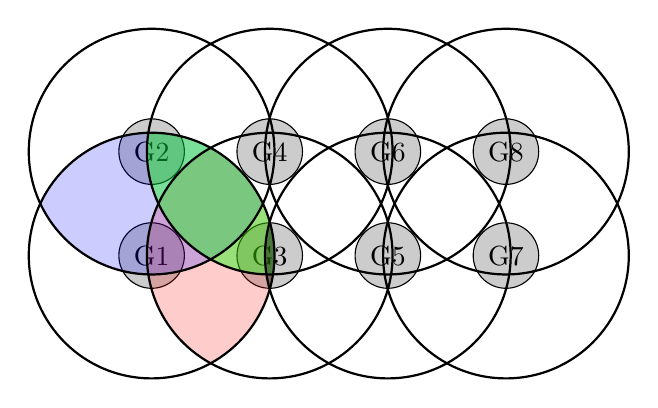
\begin{tikzpicture}[scale=0.6]
\node[circle,draw=black,fill=white!80!black,minimum size=5] (1) at (0,0)     {G1} ;
\node[circle,draw=black,fill=white!80!black,minimum size=5] (3) at (2.5,0)   {G3};
\node[circle,draw=black,fill=white!80!black,minimum size=5] (5) at (5,0)     {G5};
\node[circle,draw=black,fill=white!80!black,minimum size=5] (7) at (7.5,0)   {G7};
\node[circle,draw=black,fill=white!80!black,minimum size=5] (2) at (0,2.2)   {G2};
\node[circle,draw=black,fill=white!80!black,minimum size=5] (4) at (2.5,2.2) {G4};
\node[circle,draw=black,fill=white!80!black,minimum size=5] (6) at (5,2.2)   {G6};
\node[circle,draw=black,fill=white!80!black,minimum size=5] (8) at (7.5,2.2) {G8};

\begin{scope}
  \clip (0,0)      circle(2.6);
  \fill[red,fill opacity=.2] (2.5,0)    circle(2.6);
\end{scope}
\begin{scope}
  \clip (0,0)      circle(2.6);
  \fill[blue,fill opacity=.2] (0,2.2)    circle(2.6);
\end{scope}
\begin{scope}
  \clip (0,0)      circle(2.6);
  \fill[green,fill opacity=.4] (2.5,2.2)    circle(2.6);
\end{scope}
\begin{scope}
  \clip (0,0)      circle(2.6);
  \fill[black,fill opacity=.4] (5,0)    circle(2.6);
\end{scope}

\draw[thick](0,0)      circle(2.6);
\draw[thick](2.5,0)    circle(2.6);
\draw[thick](5,0)      circle(2.6);
\draw[thick](7.5,0)    circle(2.6);
\draw[thick](0,2.2)    circle(2.6);
\draw[thick](2.5,2.2)  circle(2.6);
\draw[thick](5,2.2)    circle(2.6);
\draw[thick](7.5,2.2)  circle(2.6);

\end{tikzpicture}
\centering
\caption{Field of view of the sensors on the vertex with the overlapping field of view for sensor 1 highlighted in color}
\label{fig:fov}
\end{figure}



\begin{figure}[!ht]
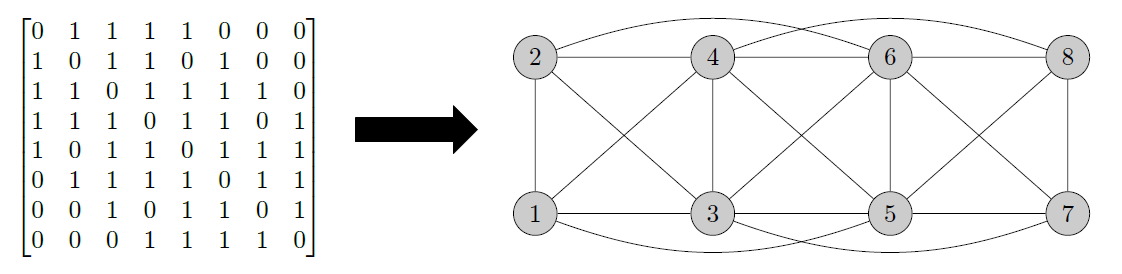
\includegraphics[width=1.0\textwidth]{./pics/adjacency.png}
\caption{Grid adjacency matrix for the grid and its corresponding adjacency graph}
\label{fig:gamGraph}


\end{figure}



\subsection{Results}
The Grid adjacency matrix for the grid and corresponding grid graph is as shown in figure \ref{fig:gamGraph}. Computed correlation matrix ($R$), its corresponding graph $G(V,E,W)$ and MST for one of the dataset are as shown in figure \ref{fig:materFig}. 
As can be seen from figure \ref{fig:corrMatrix} the correlation values between the neighboring sensors are higher than the correlation values between non-neighboring sensors. In the MST we can observe that every sensor is connected to at least one of its neighboring nodes.

\begin{figure}[!ht]
\begin{subfigure}[b]{\textwidth}
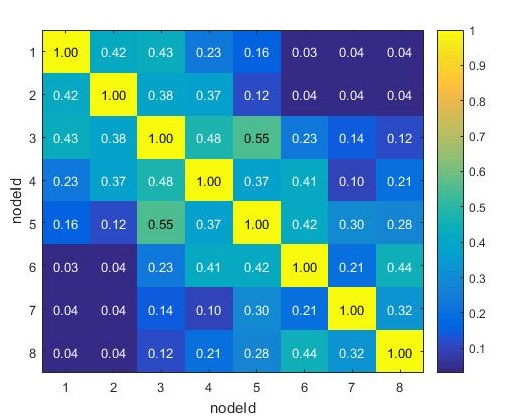
\includegraphics[scale=0.75]{./pics/correlation.jpg}
\caption{R}
\centering
\label{fig:corrMatrix}
\end{subfigure}
\hfill
\begin{subfigure}[b]{0.5\textwidth}
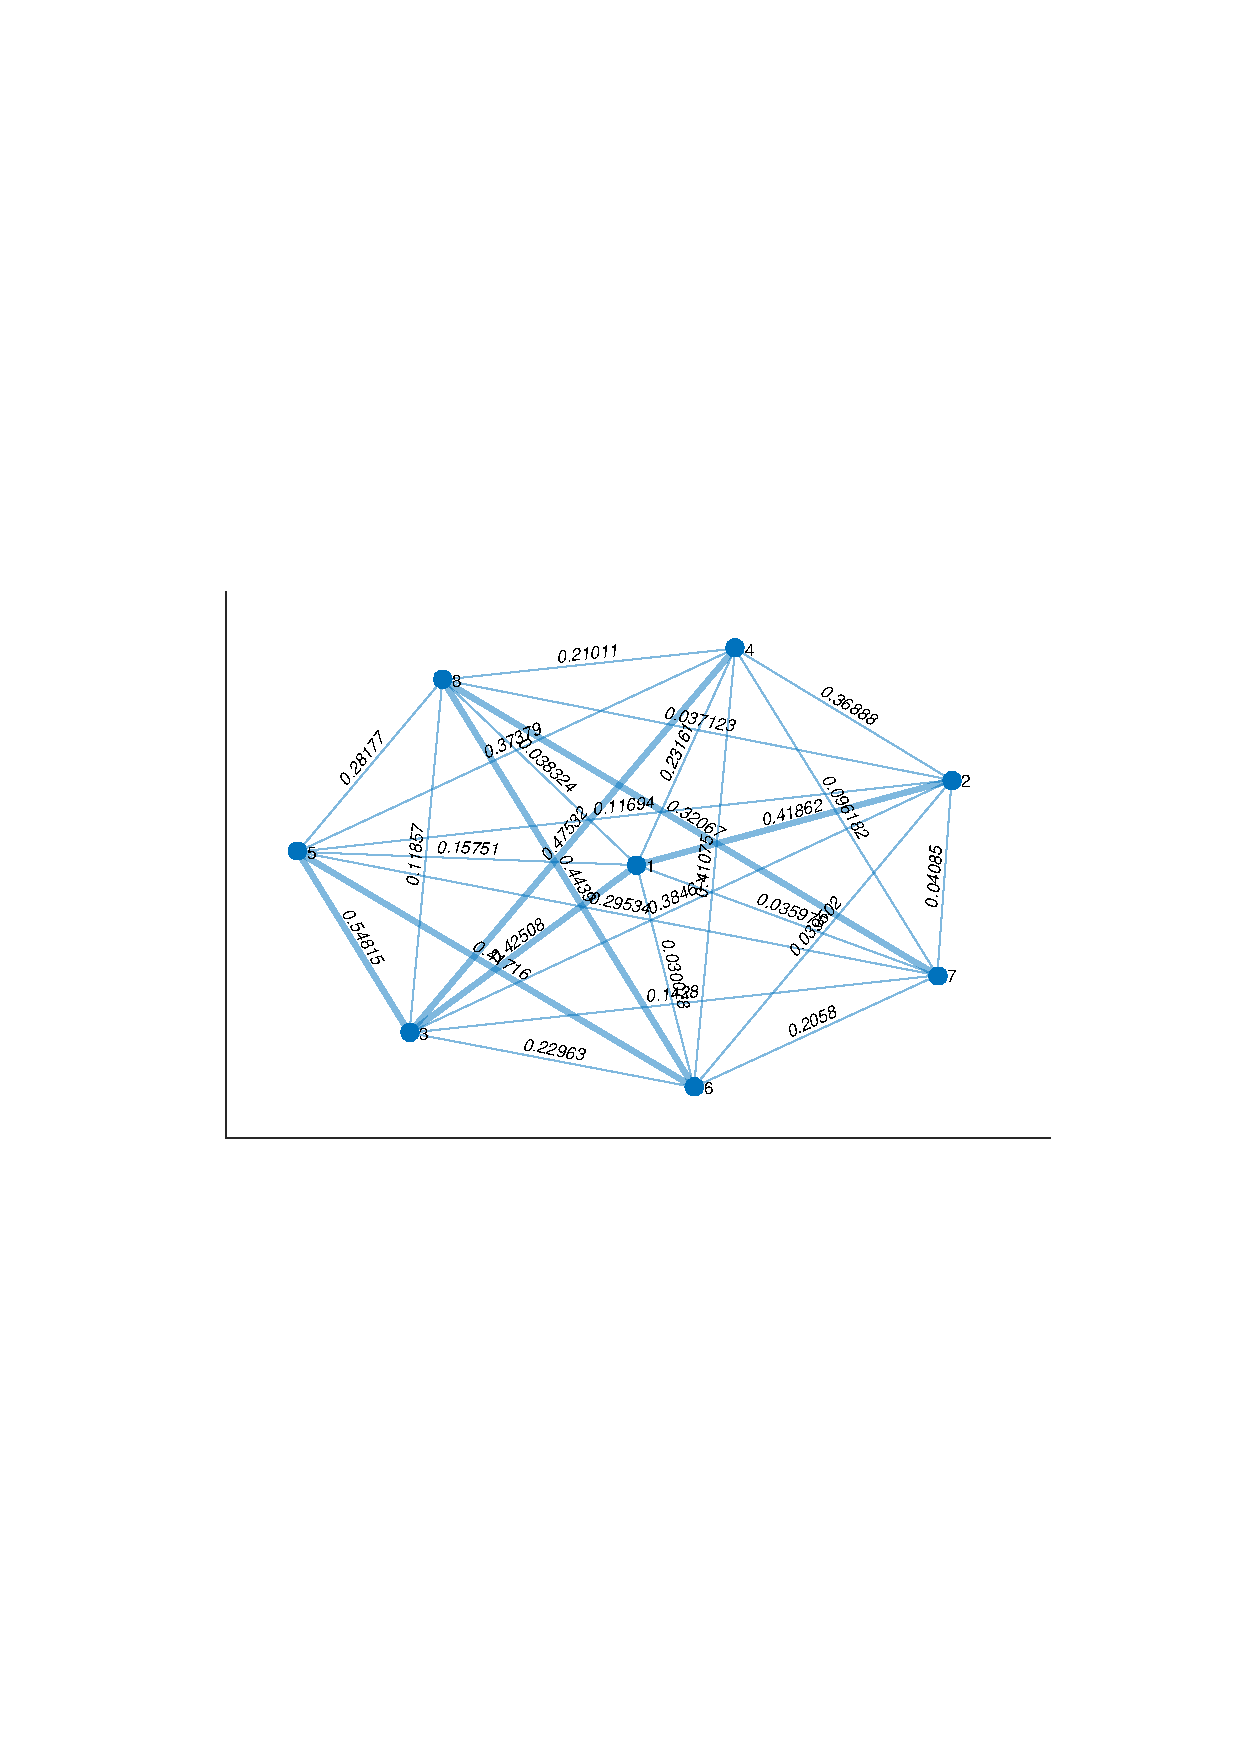
\includegraphics[scale=0.5]{./pics/corrTree.jpg}
\centering
\caption {Graph $G(V,E,W)$ for R, with MST highlighted}
\label{fig:corrMatTree}
\end{subfigure}
\hfill
\begin{subfigure}[b]{0.3\textwidth}
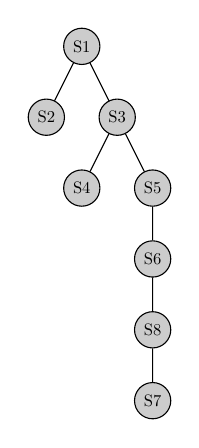
\begin{tikzpicture}[darkstyle/.style={circle,draw,fill=gray!40,minimum size=5,transform shape},scale=0.6]
\node[darkstyle]{S1}
    child{node[darkstyle]{S2}}
    child{node[darkstyle]{S3}
        child{node[darkstyle]{S4}}
        child{node[darkstyle]{S5}
                child{node[darkstyle]{S6}
                child{node[darkstyle]{S8}
                child{node[darkstyle]{S7}}
                }}}};
\end{tikzpicture}
\caption{Maximum spanning tree of $R$}
\label{fig:corrMST}
\end{subfigure}
\centering
\caption{Correlation Matrix $R$ and it's corresponding graph G and the maximum spanning tree derived from it}
\label{fig:materFig}
\end{figure}


 

Using the method described in section \ref{sec:dataLength}, we determine that the minimum data length required to compute the sensors location accurately to be 6hrs.
Hence we divide our data into blocks of 6hrs length, from which we choose 10 blocks randomly and apply our method to evaluate its performance.
10 different datasets of 6hrs each are used to evaluate the performance of our method.
For all the mappings in $M$ we compute the $GCS$ using $WGAM$. The mappings which gave the maximum $GCS$ are as shown in the figure \ref{fig:arrangement4x2}.
These mappings correspond to the actual arrangements of the sensors on the grid and its rotationally symmetrical arrangements.
We also evaluate the datasets using brute force search method and we obtain the same set of mappings as the solution that is obtained from our method. The results for both brute force and our method is presented in table \ref{tab:resHTC}.
As can be seen from table we obtain 0\% error for all the datasets. 
Further table \ref{tab:resHTC} also provides details about the number of states visited (including all the intermediate states), number of mappings between the $MST$ and grid, the number of mappings obtained as the solution from the developed method. 
Figure \ref{fig:comparision} shows the comparison between the search space for the brute force method and our method. 
The number of states visited and the number of mappings is lesser than number of  mappings which has to be checked in case of brute force search. 
\begin{table}[!ht]
\centering
\begin{tabular}{|c|c|c|c|c|c|c|c|}
\hline
\multicolumn{1}{|l|}{} & \multicolumn{4}{c|}{Graph Matching method} & \multicolumn{3}{c|}{Brute Force} \\ \hline
dataset & \begin{tabular}[c]{@{}c@{}}Number of\\ states visited\end{tabular} & Mappings & \begin{tabular}[c]{@{}c@{}}Solution \\ Mapping\end{tabular} & Error & Mappings & \begin{tabular}[c]{@{}c@{}}Solution\\  Mapping\end{tabular} & Error \\ \hline
1 & 11888 & 2744 & 4 & 0 & 40320 & 4 & 0 \\ \hline
2 & 12360 & 2744 & 4 & 0 & 40320 & 4 & 0 \\ \hline
3 & 12144 & 2664 & 4 & 0 & 40320 & 4 & 0 \\ \hline
4 & 11984 & 2752 & 4 & 0 & 40320 & 4 & 0 \\ \hline
5 & 11736 & 2592 & 4 & 0 & 40320 & 4 & 0 \\ \hline
6 & 11888 & 2744 & 4 & 0 & 40320 & 4 & 0 \\ \hline
7 & 11776 & 2736 & 4 & 0 & 40320 & 4 & 0 \\ \hline
8 & 11368 & 2664 & 4 & 0 & 40320 & 4 & 0 \\ \hline
9 & 11752 & 2656 & 4 & 0 & 40320 & 4 & 0 \\ \hline
10 & 11368 & 2664 & 4 & 0 & 40320 & 4 & 0 \\ \hline
\end{tabular}
\caption{Results obtained for experimental testbed.}
\label{tab:resHTC}
\end{table}

\begin{figure}[!ht]
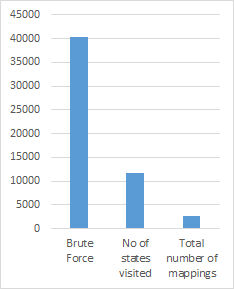
\includegraphics{./pics/comparision.png}
\caption{Comparing the search space for brute force and our method}
\label{fig:comparision}
\end{figure}

\begin{figure}[!ht]
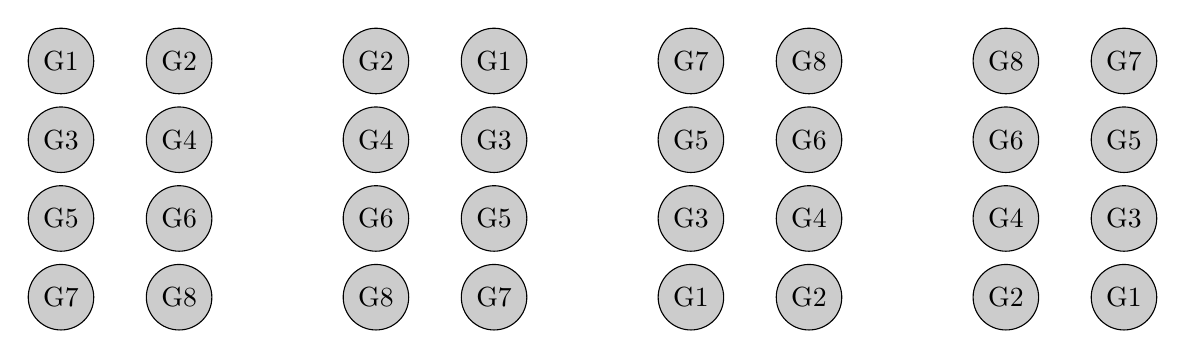
\begin{tikzpicture}
\begin{scope}
\node[circle,draw=black,fill=white!80!black,minimum size=3] (1) at (0,0)   {G7};
\node[circle,draw=black,fill=white!80!black,minimum size=3] (2) at (1.5,0) {G8};
\node[circle,draw=black,fill=white!80!black,minimum size=3] (3) at (0,1)   {G5};
\node[circle,draw=black,fill=white!80!black,minimum size=3] (4) at (1.5,1) {G6};
\node[circle,draw=black,fill=white!80!black,minimum size=3] (5) at (0,2)   {G3};
\node[circle,draw=black,fill=white!80!black,minimum size=3] (6) at (1.5,2) {G4};
\node[circle,draw=black,fill=white!80!black,minimum size=3] (7) at (0,3)   {G1};
\node[circle,draw=black,fill=white!80!black,minimum size=3] (8) at (1.5,3) {G2};
\end{scope}


\begin{scope}[shift={(4,0)}]
\node[circle,draw=black,fill=white!80!black,minimum size=3] (1) at (0,0)   {G8};
\node[circle,draw=black,fill=white!80!black,minimum size=3] (2) at (1.5,0) {G7};
\node[circle,draw=black,fill=white!80!black,minimum size=3] (3) at (0,1)   {G6};
\node[circle,draw=black,fill=white!80!black,minimum size=3] (4) at (1.5,1) {G5};
\node[circle,draw=black,fill=white!80!black,minimum size=3] (5) at (0,2)   {G4};
\node[circle,draw=black,fill=white!80!black,minimum size=3] (6) at (1.5,2) {G3};
\node[circle,draw=black,fill=white!80!black,minimum size=3] (7) at (0,3)   {G2};
\node[circle,draw=black,fill=white!80!black,minimum size=3] (8) at (1.5,3) {G1};
\end{scope}


\begin{scope}[shift={(8,0)}]
\node[circle,draw=black,fill=white!80!black,minimum size=3] (1) at (0,0)   {G1};
\node[circle,draw=black,fill=white!80!black,minimum size=3] (2) at (1.5,0) {G2};
\node[circle,draw=black,fill=white!80!black,minimum size=3] (3) at (0,1)   {G3};
\node[circle,draw=black,fill=white!80!black,minimum size=3] (4) at (1.5,1) {G4};
\node[circle,draw=black,fill=white!80!black,minimum size=3] (5) at (0,2)   {G5};
\node[circle,draw=black,fill=white!80!black,minimum size=3] (6) at (1.5,2) {G6};
\node[circle,draw=black,fill=white!80!black,minimum size=3] (7) at (0,3)   {G7};
\node[circle,draw=black,fill=white!80!black,minimum size=3] (8) at (1.5,3) {G8};
\end{scope}


\begin{scope}[shift={(12,0)}]
\node[circle,draw=black,fill=white!80!black,minimum size=3] (1) at (0,0)   {G2};
\node[circle,draw=black,fill=white!80!black,minimum size=3] (2) at (1.5,0) {G1};
\node[circle,draw=black,fill=white!80!black,minimum size=3] (3) at (0,1)   {G4};
\node[circle,draw=black,fill=white!80!black,minimum size=3] (4) at (1.5,1) {G3};
\node[circle,draw=black,fill=white!80!black,minimum size=3] (5) at (0,2)   {G6};
\node[circle,draw=black,fill=white!80!black,minimum size=3] (6) at (1.5,2) {G5};
\node[circle,draw=black,fill=white!80!black,minimum size=3] (7) at (0,3)   {G8};
\node[circle,draw=black,fill=white!80!black,minimum size=3] (8) at (1.5,3) {G7};
\end{scope}
\end{tikzpicture}
\caption{Arrangements obtained as solution for the experimental testbed}
\label{fig:arrangement4x2}
\centering
\end{figure}

%-------------------------------------------------------------WSU TOKYO TESTBED-----------------------------------------------------------------------------------------------------------------------------------%

\section{WSU Tokyo testbed}
To further validate the effectiveness of our method, we use the data from WSU smart workplace testbed\cite{cook2010detection}, a publicly available data set. The testbed called Tokyo is located in a lab,  where students perform their normal work routine. Data was collected over a period of 4 months. 
The testbed consists of 43\footnote{Sensor 38 has been ignored as no triggers were found for it throughout the dataset} motion sensors, placed as shown in the figure \ref{fig:casas}. The sensors field of view is $1.2m \times 1.2m$. In appendix \ref{app:B} we provide a detailed explanation about how we obtain the co-ordinates and the grid adjacency matrix for the testbed. The data from the WSU testbed is represented in the form of a four-tuple as shown in table \ref{tab:WSUDATA}. 
\subsection{Pre processing}
The plot of the dataset for a period of 12hrs is as shown in the figure \ref{fig:heatMap}. As can be inferred from the figure the dataset mainly consists of parts which are largely inactive. There should be a certain amount of activity happening in the space to observe correlation values between the sensors.  Also if  no activity is observed in the space it will result in all the sensors having the same values(0) and unfairly influencing the correlation values between the sensors, as correlation value is a measure of similarity between two datasets. For these reasons we filter out the parts of the data where we do not observe any trigger for a sensor for a time period of more than 3hrs. The resulting data is sampled at 100ms and is used to verify our method to find the location of the sensors.



\begin{figure}[!ht]
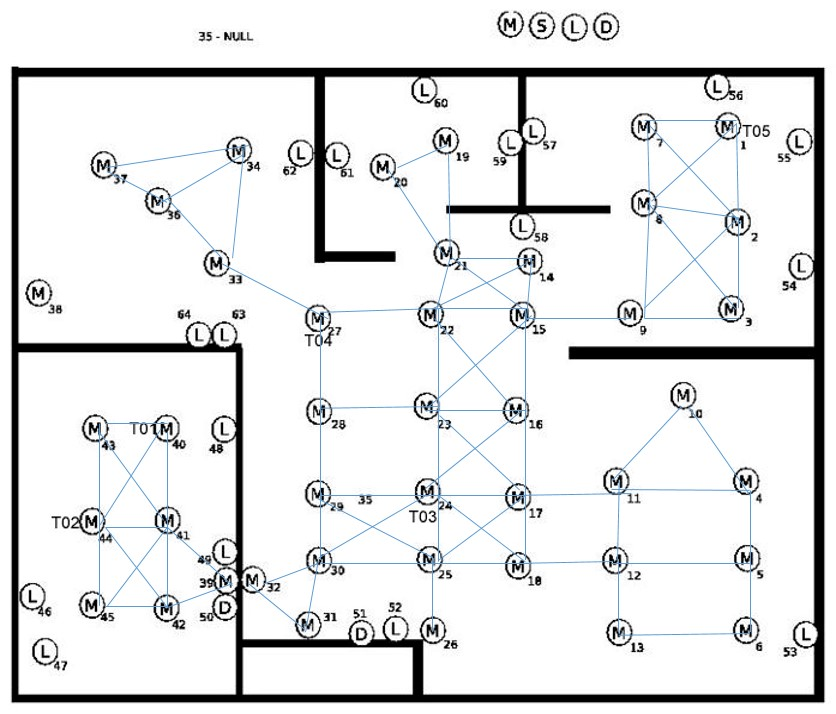
\includegraphics[scale=0.5]{./pics/LabSensorsLayout.jpg}
\centering
\caption{Floor plan for WSU CASAS office testbed, named Tokyo with adjacency marked.}
\label{fig:casas}
\end{figure}

\begin{table}[]
\centering
\caption{Data structure of the WSU data.}
\label{tab:WSUDATA}
\begin{tabular}{|c|c|c|c|}
\hline
Date       & Time            & sensor & state \\ \hline
2008-01-02 & 08:02:19.58542  & M39    & ON    \\ \hline
2008-01-02 & 08:02:19.884461 & M41    & OFF   \\ \hline
2008-01-02 & 08:02:20.297468 & M32    & ON    \\ \hline
2008-01-02 & 08:02:20.297468 & M32    & ON    \\ \hline
2008-01-02 & 08:02:20.689425 & M31    & ON    \\ \hline
2008-01-02 & 08:02:21.957307 & M44    & OFF   \\ \hline
2008-01-02 & 08:02:22.517275 & M39    & OFF   \\ \hline
\end{tabular}
\end{table}



\begin{figure}[!ht]
\includegraphics{./pics/heatMap.png}
\caption{Occupancy sensors data with 1 indicating occupancy and 0 indicating non occupancy.}
\label{fig:heatMap}
\end{figure}






\subsection{Sub layout}
Before we use the complete layout of the grid, we carry out our analysis on a $4 \times 3$ sub-layout which includes sensors 27, 22, 15, 28, 23, 16, 29, 24, 17, 30, 25, 18. This grid was chosen as it is mentioned in \cite{cook2010detection} that the region covered by these sensors is more active compared to other regions in the testbed. After processing, the data reduces to a span of 207hrs. 


\subsection{Data Length}
By using the method described in section \ref{sec:dataLength} we determine that 85hrs of processed data is required to obtain the location of the sensors accurately.  Figure \ref{fig:evst} gives an account of error for every block of data of length t, over the entire length of the data, with $t$ varying from 10 to 100 hours.
As it can be seen from the figure, for $t>85hrs$ the error observed for the blocks of data is 0. Hence to carry out our analysis we use data of length 85hrs. The required length of the data in case of WSU data set is much larger compared to that of our experimental testbed, the main reason can be because of the overlapping area in our experimental testbed is much higher than the overlapping area in Tokyo testbed, and the usage patterns are also different for both the testbed. Our experimental testbed is more active compared to Tokyo testbed.
\begin{figure}[!ht]
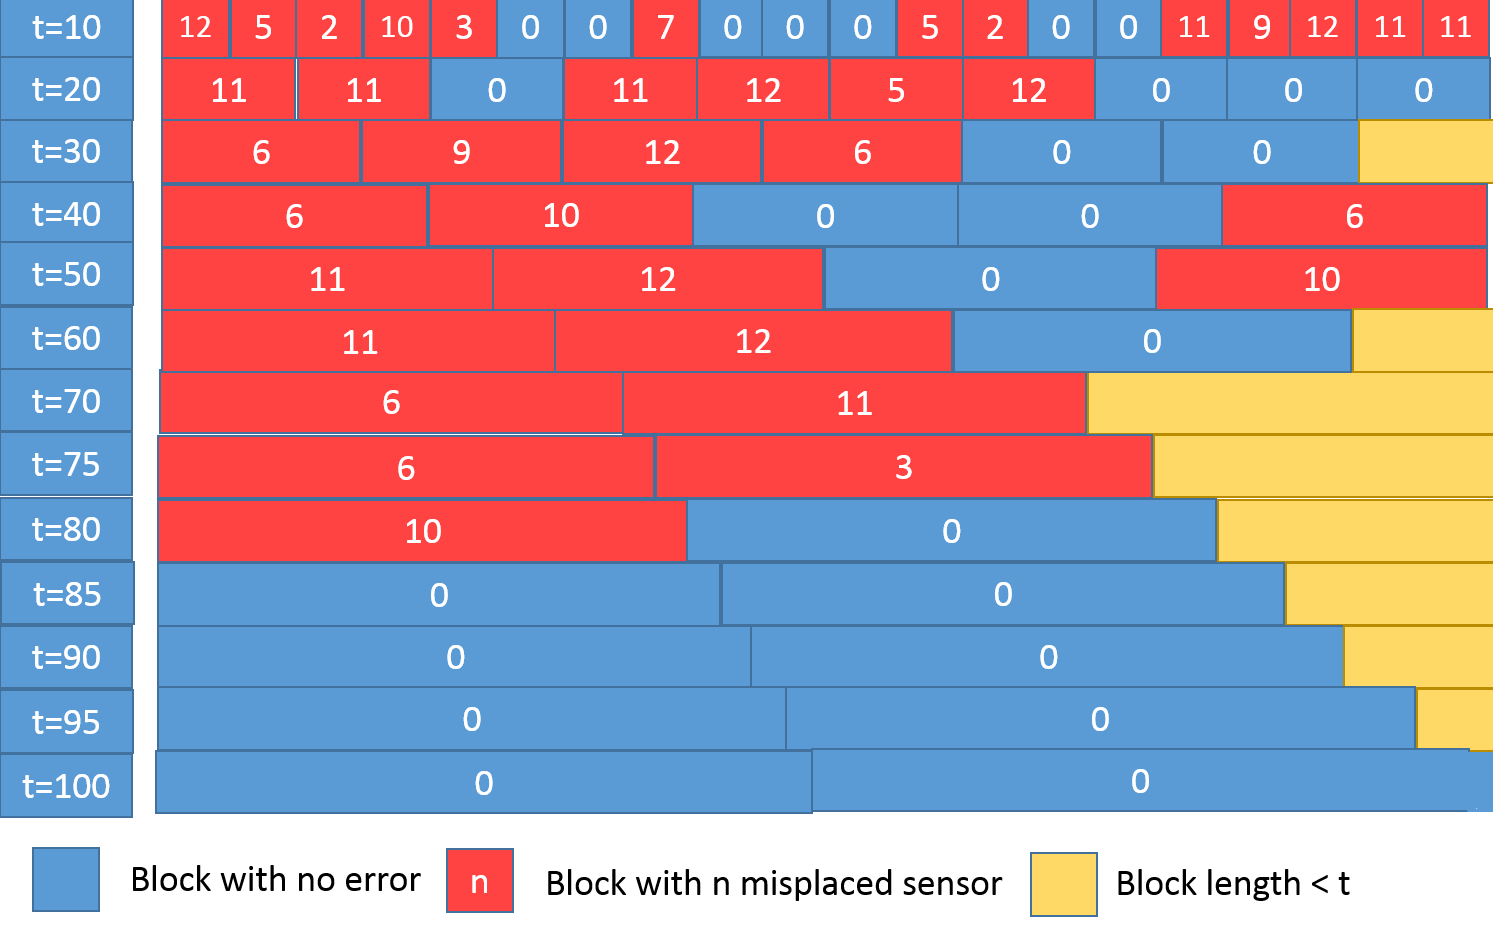
\includegraphics[scale=0.25]{./pics/errorvstime.png}
\caption{Error per block of length t for various values of t across the 200 hours of data for the $4 \times 3$ layout.}
\label{fig:evst}
\centering
\end{figure}

\subsection{Results}
Data is split into two datasets of 85hrs each. The grid graph is as shown in the figure \ref{fig:casas}. The obtained MST for both the datasets are as shown in figure \ref{fig:MST4x3}. The result obtained from the method is presented in the table \ref{tab:wsu43res}. Both brute force and our method give the same locations of the sensors as the result, but the number of arrangements that had to be checked in case of brute-force is 479001600 whereas with our method the number of mappings that had to be checked was 2120 and 1811 for dataset 1 and 2 respectively. A brute force search for the 12 sensor arrangement required approximately 27hrs to compute the results. Whereas our method needed on an average 10 seconds to compute the results. As can be seen from the table \ref{tab:resHTC} and \ref{tab:wsu43res} the number of mappings obtained is larger in the case of sensor topology of our testbed compared to a $4 \times 3$ sub-layout topology of Tokyo testbed, even though the number of sensors is more in the case of the latter. This is because the arrangement in our experimental testbed exhibits rotational symmetry. Due to which for every valid mapping between the MST and grid, the mappings which are rotationally symmetric will also be valid. Thus increasing the number of mappings.
\begin{figure}[!ht]
\centering
\begin{subfigure}[b]{0.4\textwidth}
\centering
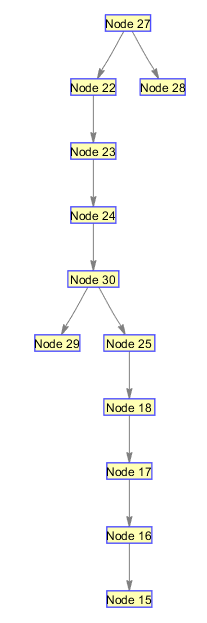
\includegraphics[scale=0.7]{./pics/MST4x3_1.png}
\hfill
\end{subfigure}
\begin{subfigure}[b]{0.4\textwidth}
\centering
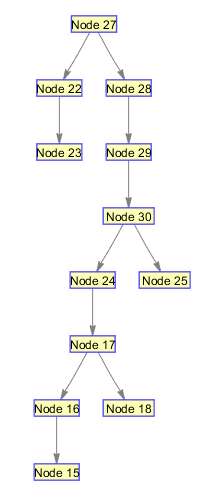
\includegraphics[scale=0.7]{./pics/MST4x3_2.png}
\hfill
\end{subfigure}
\caption{MST for the $4 \times 3$ layout}
\label{fig:MST4x3}
\end{figure}

%\begin{table}[]
%\centering
%\caption{Results obtained for WSU Tokyo testbed for $4 \times 3$ grid}
%\label{tab:wsu43res}
%\begin{tabular}{|c|c|c|c|c|c|c|c|}
%\hline
%\multicolumn{1}{|l|}{} & \multicolumn{4}{c|}{Graph matching method}                                                                                                            & %\multicolumn{3}{c|}{Brute force}                                                                                                          \\ \hline
%Dataset                & \begin{tabular}[c]{@{}c@{}}Number of \\ states visited\end{tabular} & Mappings & \begin{tabular}[c]{@{}c@{}}Solution\\  %Mappings\end{tabular} & Error & \begin{tabular}[c]{@{}c@{}}Mappings\end{tabular} & \begin{tabular}[c]{@{}c@{}}Solution\\ Mappings\end{tabular} %& Error \\ \hline
%1                      & 52664                                                               & 2120      & 1                                                            & 0     & 479001600                                                           %& 1                                                           & 0     \\ \hline
%2                      & 48909                                                               & 1811      & 1                                                            & 0     & 479001600                                                           %& 1                                                           & 0     \\ \hline
%\end{tabular}
%\end{table}


\begin{table}[!ht]
\centering
\caption{Results obtained for WSU Tokyo testbed for $4 \times 3$ grid}
\label{tab:wsu43res}
\begin{tabularx}{\textwidth}{|X|X|X|X|X|}
\hline
Dataset                                                             & \multicolumn{2}{c|}{1}       & \multicolumn{2}{c|}{2}       \\ \hline
                                                                    & Brute force & Graph Matching & Brute force & Graph Matching \\ \hline
Mappings                                                            & 479001600   & 2120           & 479001600   & 1811           \\ \hline
states visited & NA          & 52664          & NA          & 48909          \\ \hline
Solutions                                                           & 1           & 1              & 1           & 1              \\ \hline
Error                                                               & 0           & 0              & 0           & 0              \\ \hline
\end{tabularx}
\end{table}

\subsection{Complete Layout of Tokyo testbed}

After validating the $4 \times 3$ sub-layout, we apply our method to the complete layout of Tokyo testbed.

\subsection{Data length}
After applying the processing step considering all the sensors, we are left with 27hrs of data. The main reason for this is that sensor 1 and 4 are highly inactive and very fewer triggers are observed as a result majority of the data had to be filtered out. We perform our analysis on the processed data.


\subsection{Results}

We use the obtained data to compute the location of the sensors. The MST for the complete layout is as shown in figure \ref{fig:MST43}. We obtain two different mappings. 
Nodes 20 and 19 show rotational symmetry with respect to node 21 so in one arrangement nodes 19 and 20 are mapped to their respective locations in the other mapping nodes 20 and 19 locations are interchanged. As the sensors are equidistant from node 21, the locations cannot be uniquely identified using a $WGAM$. 
The result is as shown in the table \ref{tab:wsu43Resl}. We observe an error of 6.9\% as the location of three sensors are incorrectly mapped.
Brute force search for 43 sensors was not computed as the search space is of the order of $10^{52}$, and is computationally prohibitive.
While our proposed method was able to compute the sensor location within 414s $\approx$ 6mins. 
  
  

\begin{figure}
\centering
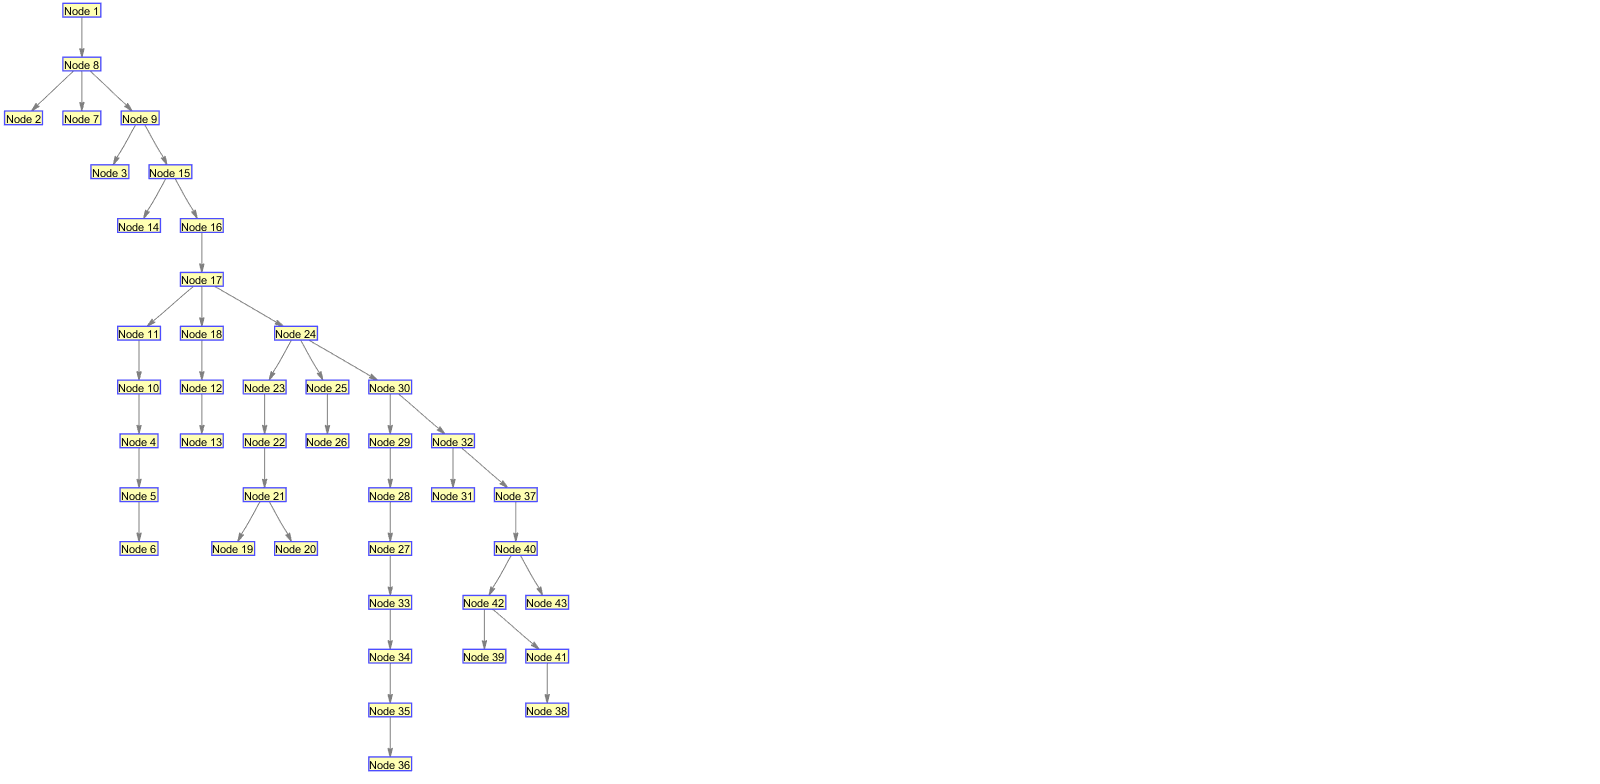
\includegraphics[width=\textwidth]{./pics/43_sensors.png}
\caption{MST for the complete layout}
\label{fig:MST43}
\end{figure}
 
 \begin{table}[!ht]
\centering
\caption{Results for the complete layout of WSU testbed}
\label{tab:wsu43Resl}
\begin{tabular}{|c|c|c|c|}
\hline
Dataset & states visited& \begin{tabular}[c]{@{}c@{}}Solution\\ Mappings\end{tabular} & Error(\%) \\ \hline
1       & 70656                                                              & 2                                                           & 6.9       \\ \hline
\end{tabular}
\end{table}

\begin{figure}[!ht]
\centering
\begin{subfigure}[b]{0.4\textwidth}
\centering
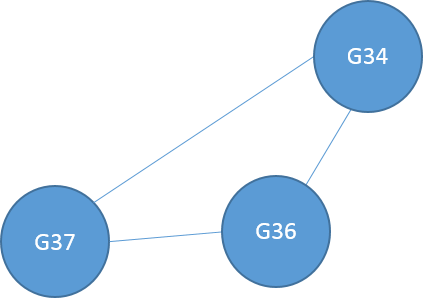
\includegraphics[scale=0.5]{./pics/grid_arr.png}
\caption{Location of vertices 34, 36 and 37 with neighboring vertices marked.}
\label{fig:true_arr}
\qquad
\end{subfigure}
\begin{subfigure}[b]{0.4\textwidth}
\centering
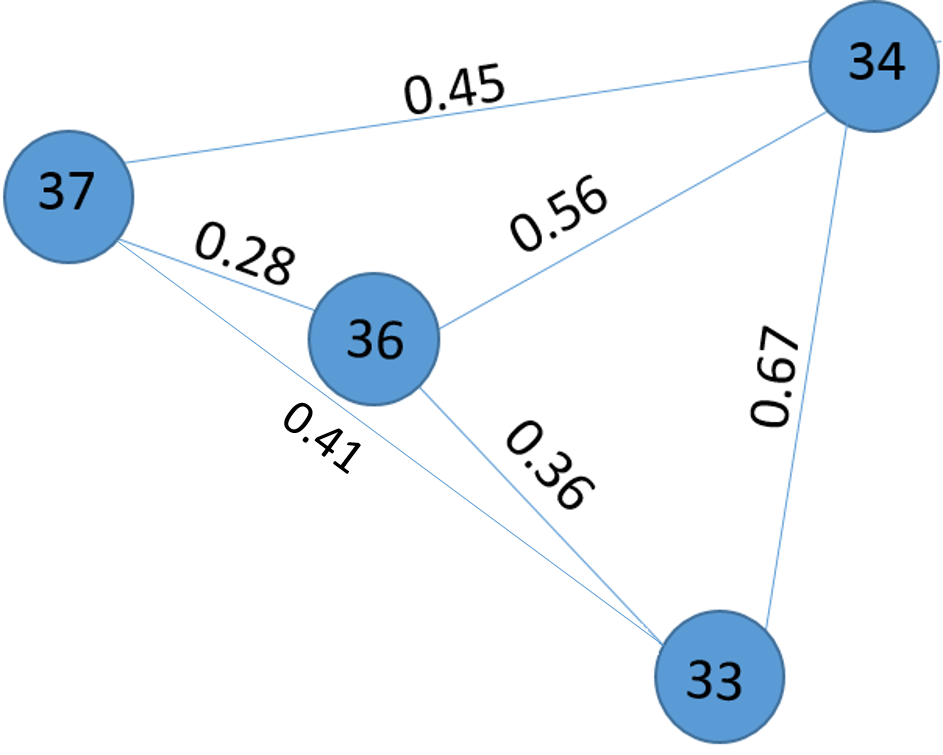
\includegraphics[scale=0.5]{./pics/true_arr.png}
\caption{Correlation value between the sensors with actual arrangement}
\label{fig:true_arr}
\qquad
\end{subfigure}
\begin{subfigure}[b]{0.4\textwidth}
\centering
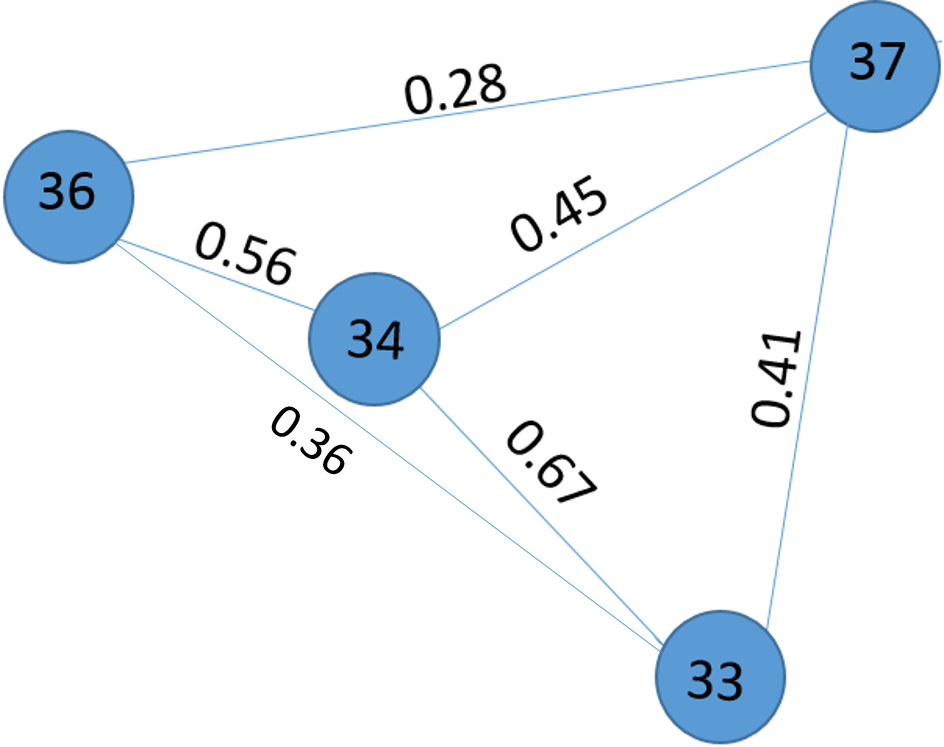
\includegraphics[scale=0.5]{./pics/computer_arr.png}
\caption{Arrangement computed by our method}
\label{fig:false_arr}
\qquad
\end{subfigure}
\begin{subfigure}[b]{0.4\textwidth}
\centering
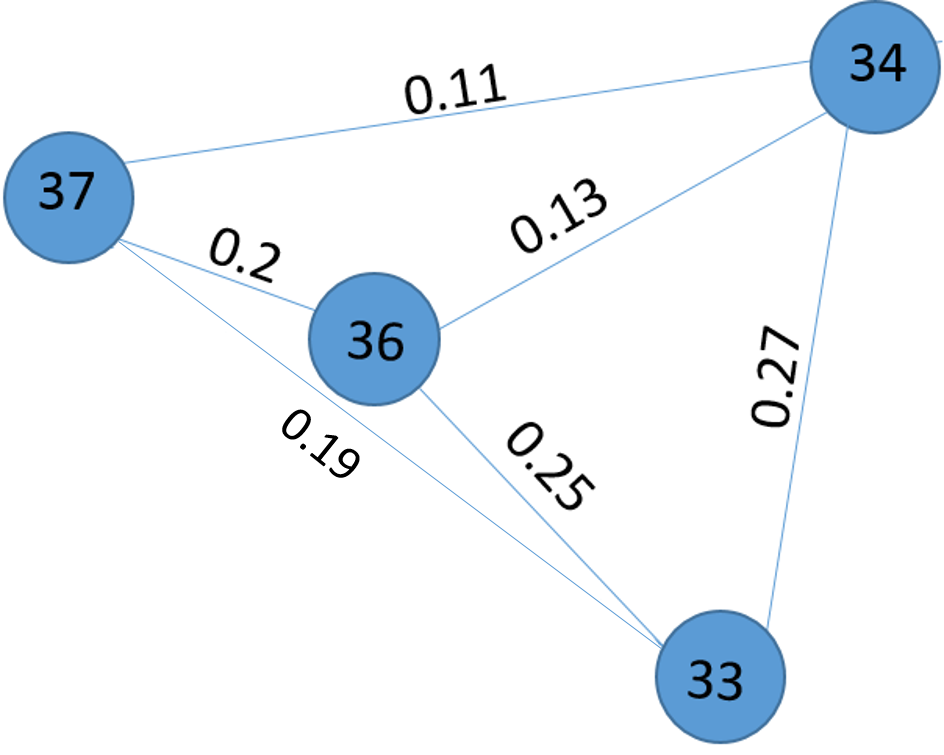
\includegraphics[scale=0.5]{./pics/long_data_arr.png}
\caption{Arrangement computed with with dataset of long duration}
\label{fig:arr}
\qquad
\end{subfigure}
\caption{Arrangement of sensors and there correlation coefficient}
\label{fig:arrangement}
\end{figure}
\subsection{Understanding the errors}
We observe error in the mappings of sensors S34, S36 and S37. Senors S34, S36 and S37 are mapped to the grid locations G36, G37 and G34 respectively. The correlation values between the sensors are as shown in the figure \ref{fig:true_arr} and the positions of the sensors obtained from our method is as shown in the figure \ref{fig:false_arr}. Since we are computing $GCS$ using $WGAM$ higher correlation values are placed on the edges which are closer to each other. Among sensors S34, S36 and S37, the maximum correlation is observed between the sensors S34 and S36. The edge with the maximum weight (vertices which are close) is between vertices G36 and G37. Therefore sensors S34 and S36 are to be placed on vertices G36 and G37 and the remaining sensor S37 will be placed on G34. The next step would be to identify which sensor should be placed on which vertex out of the two. This is decided by looking at the correlation values with sensor S37 placed on vertex G34, weight of edge (G36, G34) is greater than the weight of edge (G34,G37). Therefore sensors with higher correlation with S37 will be placed on vertex G36, which in this case would be S34. Thus we get the arrangement computed in figure \ref{fig:false_arr}.


One of the reasons for such distribution of correlation can be due to the short duration of the sensor data available. Therefore to verify, we consider only these 3 sensors and apply the preprocessing step for the parent dataset. We get resultant data of around 97hrs. Using this data we compute the correlation values. The values obtained are as shown in the figure \ref{fig:arr}. For which when the $GCS$ is calculated using $WGAM$, the maximum value of $GCS$ corresponds to the actual arrangement as shown in figure \ref{fig:arr}. Confirming that the error was caused due to the shortage of data.


\section{Summary}

In this chapter, we present the results obtained for the proposed method. Table \ref{tab:resSummary} summarizes the results for our experimental testbed and the Tokyo testbed. As can be seen, the proposed method is able to determine the locations of the sensors with no error for our experimental testbed and sub layout of Tokyo testbed. For the complete layout of the testbed, we obtain an error with respect to the location of three sensors, on further investigation we see that the main reason for the error is due to the shortage of the data. From our analysis, we can conclude that the accuracy of the results mainly depends on the data length and the level of activity happening in the space under consideration. We also see that the amount of data required for analysis becomes more if the overlapping region between the sensors are less.


\begin{table}[]
\centering
\caption{Search space comparison of brute force and our method}
\label{tab:resSummary}
\begin{tabular}{|c|c|c|c|}
\hline
Testbed                & \begin{tabular}[c]{@{}c@{}}Brute force \\ Mappings\end{tabular} & \begin{tabular}[c]{@{}c@{}}Graph matching\\  mappings\end{tabular} & Error(\%) \\ \hline
Experimental testbed   & 40320                                                           & 2696                                                               & 0         \\ \hline
Tokyo (sublayout)      & 479001600                                                       & 1966                                                               & 0         \\ \hline
Tokyo(complete layout) & $6.04 \times 10^{52}$                                           & 70656                                                              & 6.9       \\ \hline
\end{tabular}
\end{table}


















